\section{Using GIT}
\label{research:UsingGIT}
\textbf{source:} \cite{IntroductionGitVS}
Git is a distributed version control system used to track changes in source code during software development. It allows multiple developers to collaborate, manage revisions, and maintain a history of changes. Git enables branching, merging, and working offline, making it flexible and efficient. It is widely used in software projects and integrates with platforms like GitHub and GitLab for remote collaboration.

My IDE (integrated development environment - code editor) of choice is Visual Studio Code which thankfully has very tight integration with GIT. Whilst each tutorial sets this up separately here is the process I used: \cite{IntroductionGitVS} - the official ide documentation.

Within my ide I now have a tab showing me the status of my Git repository (the name for a project on git), the changes tab shows me changes that have been made since the last commit (the last time my code was 'pushed' the central master branch), within this I can choose for different files to be excluded from a push,  automatically pushed or be ignored (such as my database which for security reasons stays locally on my device).

Below that view is the list of past commits I have been along with the comments, should I want to revert a change I previously made I can simply pull it from a prior commit, copy the change and then push it back to update the master. I can also setup multiple 'branches'. A branch may be for a backend change that is in progress but shouldn’t yet be committed to the 'master' branch which is what each user will see, by using branches I can work on separate features without making breaking changes and simply 'merge' the final code into the master branch for integration / distribution
 


\begin{figure}[H]
    \centering
    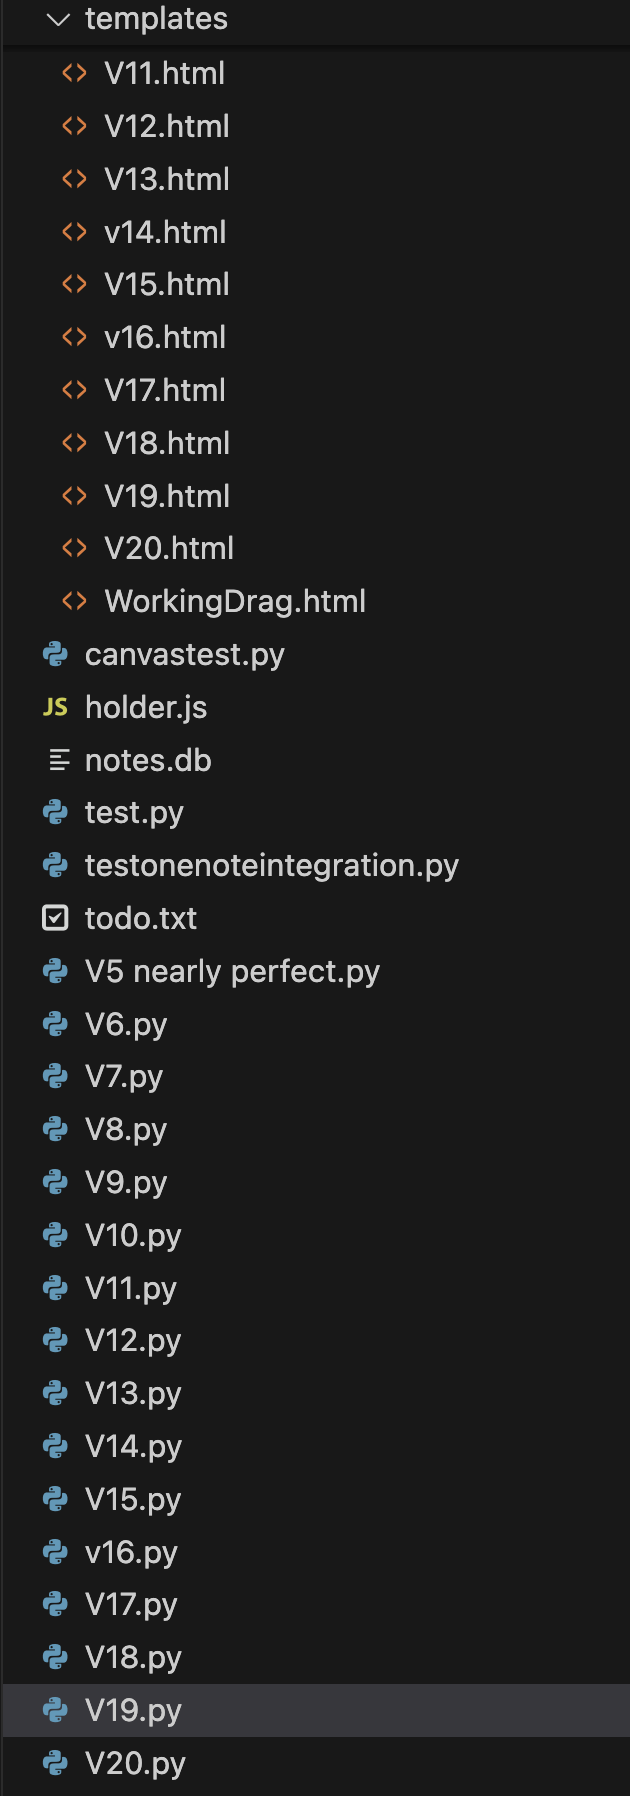
\includegraphics[width=0.2\textwidth]{Research/12_UsingGIT/media/preGit.png}
    \caption{Before using Git I had a file for each major version}
\end{figure}

\begin{figure}[H]
    \centering
    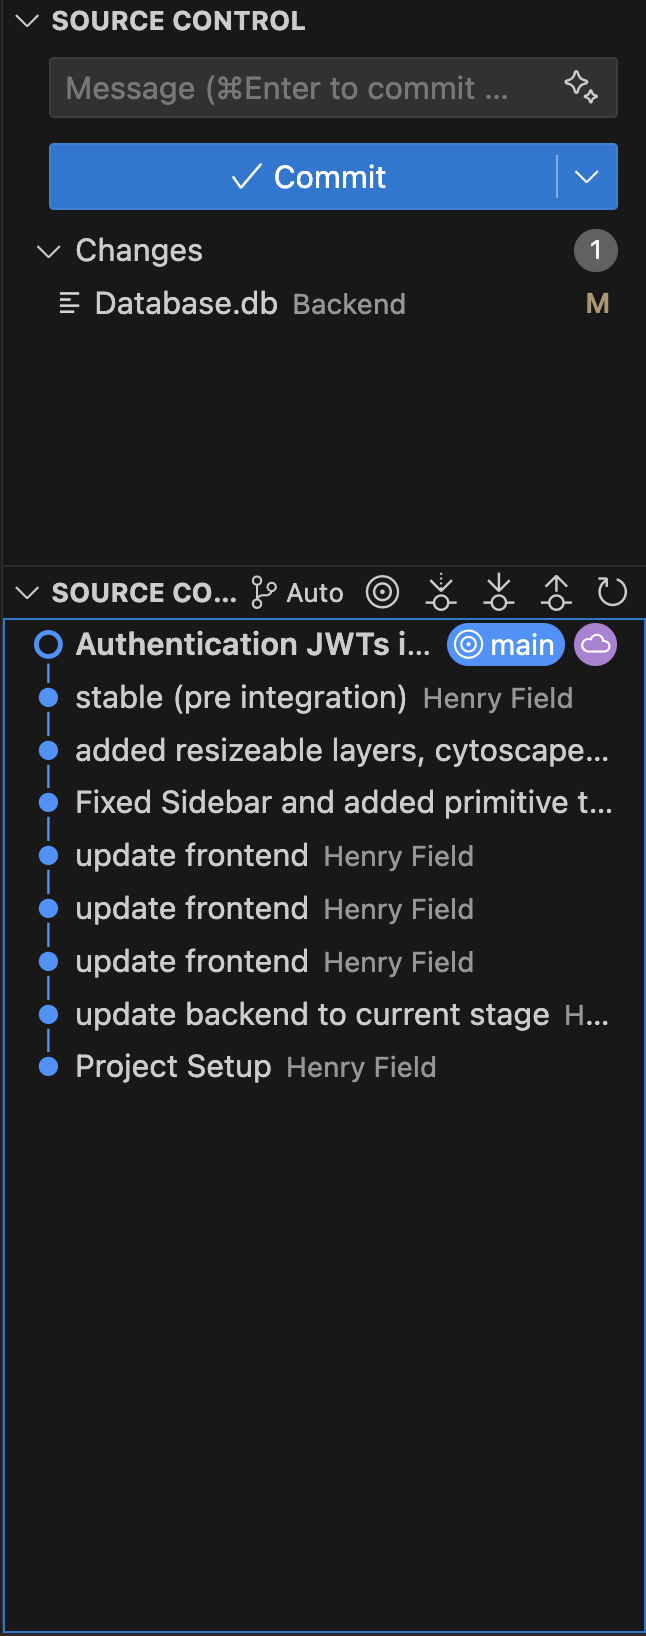
\includegraphics[width=0.2\textwidth]{Research/12_UsingGIT/media/versionControl.png}
    \caption{Using Git I can now track changes to my code and revert them if needed}
\end{figure}

